\documentclass{article}[12pt]

%----- Math ---------------------------------------------
\usepackage{amsmath}   
\usepackage{mathrsfs}      
\usepackage{mathtools}       
\usepackage{amssymb}   
\usepackage{amsthm}   
\usepackage{esint}     
\usepackage{resmes} 
\usepackage{stackengine}
\usepackage{amsfonts}
\usepackage{stmaryrd}
\usepackage{dsfont}



%----- Design ------------------------------------------- 
\usepackage{lastpage}                              
\usepackage{enumitem}
\usepackage{multirow}


%----- Intestazioni ---------------------------------------
\usepackage{fancyhdr}
\pagestyle{fancy}
\fancyhf{} % Clear all headers and footers
\fancyhead[R]{\nouppercase{\leftmark}} % Header right on all pages
\fancyfoot[C]{\thepage} % Footer center, page number
\setlength{\headheight}{14.5pt}

% Pacchetto titlesec per personalizzare i titoli dei capitoli
\usepackage{titlesec}

% Comando per settare l'intestazione correttamente per l'introduzione
\newcommand{\chapterwithintroduction}[1]{
	\chapter*{#1}
	\addcontentsline{toc}{chapter}{#1}
	\markboth{#1}{}
}

%----- Pacchetti Disegno --------------------------------
\usepackage{tikz}
\makeatother 
\usetikzlibrary{3d,perspective}
\usetikzlibrary{patterns}
\usetikzlibrary{arrows,calc,patterns}
\usepackage{tikz-cd}
\usepackage{graphicx}
\usepackage{thmtools}
\usepackage{xcolor}
\usepackage[all]{xy}        
\usetikzlibrary{decorations.markings}
\usetikzlibrary{hobby}
\usepackage{pgfplots}
\pgfplotsset{compat=1.18}


%----- Symbols -----------------------------------------
\input{symbols}

%----- Hyperref ------------------------------------------
\usepackage{nameref}
\usepackage{csquotes}
\usepackage{hyperref}
\hypersetup{
	colorlinks=true,
	linkcolor=black, % Color for normal internal links
	filecolor=black, % Color for file links
	urlcolor=blue, % Color for external links
	citecolor=blue % Color for citations
}
\usepackage{cleveref} 


% -----Ambienti matematici-------------------------------
\theoremstyle{plain}
\newtheorem{thm}{Theorem}[section]
\newtheorem*{thm*}{Theorem}
\newtheorem{prop}[thm]{Proposition}
\newtheorem{cor}[thm]{Corollary}
\newtheorem{lemma}[thm]{Lemma}
\newtheorem{claim}{Claim}
\theoremstyle{definition}
\newtheorem{defi}[thm]{Definition}
\newtheorem{axiom}{Axiom}
\theoremstyle{remark}
\newtheorem{rmk}[thm]{Remark}
\newtheorem{ex}[thm]{Example}
\newtheorem{exercise}{Exercise}


%------BIBLIOGRAFIA-----------
\usepackage[style=alphabetic, backend=biber]{biblatex}
% Definizione di un nuovo driver per nascondere URL e DOI
\AtEveryBibitem{
 	\clearfield{url} % Nasconde l'URL
 	\clearfield{doi} % Nasconde il DOI
 	\clearfield{isbn} % Nasconde ISBN
 	\clearfield{issn} % Nasconde ISSN
 	\clearfield{note} % Nasconde le note
}
\addbibresource{biblio.bib}
\title{Christodoulou-Yau theorem for higher genus}
\author{Andrea Martelli}
\date{May 2025}

\begin{document}

\maketitle

\section{Introduction}

It holds the following theorem, proved by D. Christodoulou and S.T. Yau:
\begin{thm}[Christodoulou, Yau]\label{thm: Christodoulou-Yau}
    Let \((M^3,g)\) be a Riemannian 3-manifold and let \(\Sigma^2 \subset (M^3,g)\) be volume-preserving stable CMC sphere. Then
    \begin{equation}\label{eq: CY eq}
        16\pi - H^2|\Sigma| \ge \frac{2}{3}\int_\Sigma (R^M+|h^\circ|^2) \ \dif \sigma.
    \end{equation}
    In particular, if \((M,g)\) has positive scalar curvature \(R^M\ge 0\), the Hawking mass of \(\Sigma\) is non-negative:
    \[
        m_{\mathrm{Haw}}(\Sigma) \coloneq \sqrt{\frac{|\Sigma|}{16\pi}}\left( 1 - \frac{1}{16\pi}\int_\Sigma H^2 \dif \sigma \right) \ge 0.
    \]
\end{thm}
The importance of this result is due to a theorem of Huisken and Yau \cite{HuiskenYau_CenterMass}: every asymptotically flat\footnote{A complete 3-manifold \((M,g)\) is \emph{asymptotically flat} if there is a compact subset \(K \subset M\), a positive number \(R>0\) and a diffeomorphism \(\vp \colon \R^3 \setminus B_R(0) \to M\setminus K\) such that if \(g_{ij} \dif x^i\dif x^j = \vp^*g\) on \(\R^3\setminus B_R(0)\), then
\[
    g_{ij}= \left(1+ \frac{2m}{r} \right) \delta_{ij} + O(r^{-2}).
\]
The charts like \((M\setminus K, \vp^{-1})\) are called \emph{AF charts}.} 3-manifold \((M,g)\) admits a foliation of the asymptotically flat end by CMC-stable 2-spheres \(\{\Sigma_r\}_{r>R}\). Then we could define a notion of total mass taking the limit of the Hawking mass of these CMC-stable 2-spheres when \(R \to +\infty\). Turns out that is coincide with the Arnowitt–Deser–Misner (ADM) mass\footnote{
    Fix an AF chart \((M\setminus K, x^1,\dots, x^n)\). Then the ADM mass of \((M,g)\) is:
    \[
        m_{ADM}(M,g) \coloneq \frac{1}{2(n-1)|\Sp^{n-1}|}\lim_{r \to \infty} \int_{\{|x|=r\}} \left(\frac{\de g_{ij}}{\de x^i}- \frac{\de g_{ii}}{\de x^j} \right) \frac{x^i}{|x|} \ \dif \sigma_e,
    \]
    where \(\dif \sigma_e\) is the area element on \(\{|x|=r\}\) induced by the Euclidean metric of \(\R^n\setminus B_R(0)\).
}
\[
    m_{\mathrm{ADM}}(M,g) = \sup_{r>R} m_{\mathrm{Haw}}(\Sigma_r).
\]
Given this facts, as a corollary of Christodoulou-Yau theorem we get the positive mass theorem. 

\begin{cor}[Positive mass theorem]
    Let \((M^3,g)\) be an asymptotically flat Riemannian 3-manifold with non negative scalar curvature \(R_g \ge 0\). Then the ADM mass is non negative.
\end{cor}

In this note, we extend Theorem\ref{thm: Christodoulou-Yau} to orientable surfaces \(\Sigma\) of any genus. 

\begin{thm}\label{thm: Christodoulou-Yau for higher genus}
    Let \((M^3,g)\) be a Riemannian 3-manifold and let \(\Sigma^2 \subset (M^3,g)\) be volume-preserving stable CMC surface of genus \(k\). Then
    \begin{itemize}
        \item if \(k\) is even,
        \[
        16\pi - H^2|\Sigma| \ge \frac{2}{3}\int_\Sigma (R^M+|h^\circ|^2) \ \dif \sigma;
        \]  
        \item if \(k\) is odd,
        \[
        \frac{64\pi}{3} - H^2|\Sigma| \ge \frac{2}{3}\int_\Sigma (R^M+|h^\circ|^2) \ \dif \sigma.
        \]
    \end{itemize}
\end{thm}

The proof of Theorem~\ref{thm: Christodoulou-Yau for higher genus}, which will be given in Section~\ref{sec: Christodoulou Yau for higher genus}, is an adaptation of the proof of Theorem~\ref{thm: Christodoulou-Yau}. Specifically, the idea is to use the CMC-stability inequality with zero-average test functions, that will be constructed using two key results:
\begin{enumerate}[label=(\roman*)]
    \item Brill-Noether theory,
    \item Hersch's balancing trick.
\end{enumerate}

Let us briefly state them here. 

\begin{thm}\label{thm: corollary of Brill-Noether}
	If \((\Sigma,g)\) is a closed (compact and without boundary) oriented surface of genus \(k\), then there exists a branched conformal covering map
    \[
        \Phi \colon (\Sigma,g) \to (\Sp^2,g_{\Sp^2})
    \]
    with degree 
	\begin{equation}\label{eq: Brill-Noether bounds on the degree}
		\deg(\Phi) = \begin{cases}
			1+k/2 & \text{if }k \text{ is even}\\
			3/2+ k/2 &\text{if }k \text{ is odd}.
		\end{cases}
	\end{equation}
\end{thm}

\begin{defi}
    A \emph{branched conformal covering map} is a smooth map
    \[
    \Phi \colon (\Sigma_1,g_1) \to (\Sigma_2,g_2)
    \] 
    between oriented closed surfaces such that there is a finite set \(\Gamma\subset \Sigma_1\) (whose points are called \emph{branch points}) with finite image and 
    \[
    \Phi \colon (\Sigma_1\setminus\Gamma,g_1) \to (\Sigma_2\setminus \Phi(\Gamma),g_2)
    \] 
    is a conformal covering map.  
\end{defi}

The proof of Theorem~\ref{thm: corollary of Brill-Noether} is a consequence of the Brill-Noether Theorem~\ref{thm: Brill-Noether}, and it is postponed to the appendix of this note.

\begin{lemma}[Hersch's balancing trick]\label{lem: Hersch trick}
	Let \(\Sigma^2 \subset (M^3,g)\) be a closed oriented surface and a map \(\Phi \colon (\Sigma,g) \to (\Sp^2,g_{\Sp^2})\). Then there exists a conformal diffeomorphism \(\gamma \in \mathrm{Conf}(\Sp^2,g_{\Sp^2})\) such that 
	\begin{equation}\label{eq: x_i orthogonal to phi_1}
		\int_\Sigma (x^i \circ \gamma \circ \Phi) \ \dif \sigma = 0
	\end{equation}
	for each \(i=1,2,3\), where \(x^i\) is the restriction to \(\Sp^2 \subset \R^3\) of the \(i\)-th coordinate of \(\R^3\).
\end{lemma}

We will provide a proof in Section~\ref{sec: Hersch's trick}.

In Section~\ref{sec: CMC-stabile with positive genus}, we will try to test Theorem~\ref{thm: Christodoulou-Yau for higher genus} looking for some CMC-stable surfaces of positive genus. 


\section{Christodoulou-Yau theorem for higher genus}\label{sec: Christodoulou Yau for higher genus}

Before jumping in the proof of Theorem~\ref{thm: Christodoulou-Yau for higher genus}, let us point out some consequences.

In 2014, Marques and Neves \cite{MarquesNeves_Willmore} proved that for every surface \(\Sigma \subset \R^3\) with genus at least 1,
\begin{equation}\label{eq: Willmore}
    \int_\Sigma H^2 \ge 8\pi^2
\end{equation}
with equality if and only if \(\Sigma\) is a torus obtained by stereographic projecting the Clifford torus \(\Sp^1(1/\sqrt{2}) \times \Sp^1(1/\sqrt{2})\) of the round 3-sphere \(\Sp^3\). 

As an immediate consequence of Theorem~\ref{thm: Christodoulou-Yau for higher genus},
\begin{cor}
    There are no CMC-stable surfaces of genus \(k\ge 1\) in the Euclidean space \(\R^3\).
\end{cor}
\begin{proof}
    Suppose by contradiction that there exists a CMC-stable surface \(\Sigma \subset \R^3\) of genus \(k\ge 1\). Suppose that \(k\) is odd. Then by \eqref{eq: Willmore} and Theorem~\ref{thm: Christodoulou-Yau for higher genus},
    \begin{align*}
        8\pi^2 &\le \int_\Sigma H^2 \ \dif \sigma \le -\frac{2}{3}\int_\Sigma |h^\circ|^2 \ \dif \sigma + \frac{64\pi}{3} \\
        & \le \frac{64\pi}{3},
    \end{align*}
    a contradiction. If \(k\) is even, in the same way we can get \(8\pi^2 \le 16\pi\), a contradiction. \qedhere
\end{proof}
\begin{proof}[Proof of Theorem~\ref{thm: Christodoulou-Yau for higher genus}]
    Let \(\Phi \colon (\Sigma,g) \to (\Sp^2,g_{\Sp^2})\) as in Theorem~\ref{thm: corollary of Brill-Noether}. By Lemma~\ref{lem: Hersch trick}, up to consider \(\gamma \circ \Phi\) for some conformal diffeomorphism \(\gamma \in \mathrm{Conf}(\Sp^2,g_{\Sp^2})\), we can assume that 
    \begin{equation*}
		\int_\Sigma (x^i \circ \Phi) \ \dif \sigma = 0.
	\end{equation*}
    Therefore we can use the CMC-stability inequality on each function \(x^i \circ \Phi\)
    \begin{equation*}
        \int_\Sigma |\nabla_g (x^i \circ \Phi)|^2 \dif \sigma \ge \int_\Sigma \left[ |h|^2 + \Ric^M(\nu,\nu)\right](x^i \circ \Phi)^2 \dif \sigma .
    \end{equation*}
    Observe that since \(\Phi\) has value on the unit sphere of \(\R^3\),
    \begin{equation}\label{eq: sum (xi.Phi)^2=1}
	   \sum_{i=1}^3 (x^i \circ \Phi)^2=1,
    \end{equation}
    thus summing over \(i\) the previous inequality we get
    \begin{equation}\label{eq: CMC-stability}
        \sum_{i=1}^3\int_\Sigma |\nabla_g (x^i \circ \Phi)|^2 \dif \sigma \ge \int_\Sigma \left[ |h|^2 + \Ric^M(\nu,\nu)\right] \ \dif \sigma .
    \end{equation}
    
    Now we want to rewrite both sides of the inequality.

    First consider the left hand side.

    \begin{claim} \label{claim: energy and conformal diffeo}
    For any function \(u \in C^\infty(\Sp^2)\),
        \[
            \int_\Sigma |\nabla_g(u \circ \Phi)|^2_{g} \dif \sigma_g = \deg(\Phi)\int_{\Sp^2} |\nabla_{g_{\Sp^2}} u|^2_{g_{\Sp^2}} \dif \sigma_{\Sp^2}.
        \]
    \end{claim}
    \begin{proof}[Proof of Claim~\ref{claim: energy and conformal diffeo}]
        By definition of degree, 
        \[
            \int_\Sigma |\nabla_{\Phi^*g_{\Sp^2}}(u \circ \Phi)|^2_{\Phi^*g_{\Sp^2}} \dif \sigma_{\Phi^*g_{\Sp^2}} = \deg(\Phi)\int_{\Sp^2} |\nabla_{g_{\Sp^2}} u|^2_{g_{\Sp^2}} \dif \sigma_{\Sp^2}.
        \]
        Since \(\Phi\) is conformal away from a finite set \(S\subset \Sp^2\), there is a smooth function \(\lambda \colon \Sigma\setminus \Gamma \to \R\setminus\{0\}\), where \(\Gamma=\Phi^{-1}(S)\), such that
        \[
            g = \lambda^2\Phi^* g_{\Sp^2} \qquad \text{on }\Sigma \setminus \Gamma.
        \]
        To prove the claim, it's enough to show that
        \begin{equation}\label{eq: Riemannian area element under conformal changes}
            \dif \sigma_g = \lambda^2 \dif \sigma_{\Phi^*g_{\Sp^2}}
        \end{equation}
        and that for any \(v \in C^\infty(\Sigma \setminus \Gamma)\)
        \begin{equation}\label{eq: gradient under conformal changes}
            |\nabla_g v|^2_g = \lambda^{-2}|\nabla_{\Phi^*g_{\Sp^2}} v |^2_{\Phi^*g_{\Sp^2}}.
        \end{equation}

        Let's prove \eqref{eq: Riemannian area element under conformal changes}. Fix some coordinates \((U,x^i)\) on \(\Sigma \setminus \Gamma\) and write \(g= g_{ij} \dif x^i \otimes \dif x^j\) and \(\Phi^*g_{\Sp^2} = \widetilde{g}_{ij}\dif x^i \otimes \dif x^j\). Then
        \[
            g_{ij} = \lambda^2 \widetilde{g}_{ij}.
        \]
        so
        \begin{align*}
            \dif \sigma_{g} &= \sqrt{\det(g_{ij})} \ \dif x^1 \wedge \dif x^2\\
            &= \sqrt{\det(\lambda^2\widetilde{g}_{ij})} \ \dif x^1 \wedge \dif x^2\\
            &= \lambda^2 \sqrt{\det(\widetilde{g}_{ij})} \ \dif x^1 \wedge \dif x^2 = \lambda^2 \dif \sigma_{\Phi^*g_{\Sp^2}}.
        \end{align*}

        Now let's prove \eqref{eq: gradient under conformal changes}. Fix coordinates as above and observe that
        \[
            g^{ij} = \lambda^{-2} \widetilde{g}^{ij}.
        \]
        Recall that
        \[
            |\nabla_g u|_g^2 = g_{ij}(\nabla_g u)^i (\nabla_g u)^j = g_{ij}g^{ik}g^{j\ell}\frac{\de u}{\de x^k}\frac{\de u}{\de x^\ell},
        \] 
        and similarly
        \[
            |\nabla_{\Phi^*g_{\Sp^2}} u|_{\Phi^*g_{\Sp^2}}^2 = \widetilde{g}_{ij}\widetilde{g}^{ik}\widetilde{g}^{j\ell}\frac{\de u}{\de x^k}\frac{\de u}{\de x^\ell} = \lambda^{-2} g_{ij}g^{ik}g^{j\ell}\frac{\de u}{\de x^k}\frac{\de u}{\de x^\ell}.
        \]
        Therefore
        \[
            |\nabla_g u|^2_{g} = \lambda^{-2} |\nabla_{\Phi^*g_{\Sp^2}} u|_{\Phi^*g_{\Sp^2}}^2.
        \]

        This completes the proof of the claim. \qedhere
    \end{proof}

    Using Claim~\ref{claim: energy and conformal diffeo}, the left hand side of \eqref{eq: CMC-stability} becomes
    \begin{align}\label{eq: energy computation}
        \sum_{i=1}^3\int_\Sigma |\nabla_g (x^i \circ \Phi)|^2 \dif \sigma &= \deg(\Phi)\int_{\Sp^2} \sum_{i=1}^3 |\nabla_{g_{\Sp^2}} x^i|^2_{g_{\Sp^2}} \dif \sigma_{\Sp^2} \nonumber \\
        &= \deg(\Phi)\int_{\Sp^2} \sum_{i=1}^3 \left|e^i-(e^i\cdot x)x\right|^2_{g_{\R^3}} \dif \sigma_{\Sp^2}(x) \nonumber\\
        &= \deg(\Phi)\int_{\Sp^2} 2 \ \dif \sigma_{\Sp^2} \nonumber\\
        &= 8\pi \deg(\Phi).
    \end{align}

    Now let us rearrange the right hand side of \eqref{eq: CMC-stability}. Using the twice contracted Gauss equation,
    \begin{align*}
        |h|^2 + \Ric(\nu,\nu) &= |h|^2 + \frac{1}{2}\left[R^M -R^\Sigma + H^2-|h|^2\right]\\
        &= \frac{1}{2}|h|^2 + \frac{1}{2}R^M -\frac{1}{2}R^\Sigma + \frac{1}{2}H^2 \\
        &=\frac{1}{2}\left(|h^\circ|^2+R^M\right) + \frac{3}{4}H^2 -\frac{1}{2}R^\Sigma.
    \end{align*}
    Using this computation and \eqref{eq: energy computation}, we can rewrite \eqref{eq: CMC-stability} as
    \begin{align*}
        8\pi \deg(\Phi) &= \int_\Sigma \frac{1}{2}\left(|h^\circ|^2+R^M\right) + \frac{3}{4}H^2 -\frac{1}{2}R^\Sigma \ \dif \sigma.
    \end{align*}
    By Gauss-Bonnet theorem
    \[
        \int_\Sigma \frac{R^\Sigma}{2} \ \dif \sigma = 2\pi \chi(\Sigma) = 2\pi(2-2k)= 4\pi-4k\pi.
    \]
    Thus 
    \begin{align*}
        \frac{1}{2}\int_\Sigma (|h^\circ|^2+R^M) \ \dif \sigma \le 8\pi \deg(\Phi) +4\pi-4k\pi - \frac{3}{4}H^2|\Sigma|. 
    \end{align*}
    Assume that \(k\) is even. Then \(\deg(\Phi) \le 1+ k/2\), so
    \begin{align*}
        \frac{1}{2}\int_\Sigma (|h^\circ|^2+R^M) \ \dif \sigma&\le 8\pi \deg(\Phi) +4\pi-4k\pi - \frac{3}{4}H^2|\Sigma|\\
        &\le 8\pi +4k\pi +4\pi -4k\pi -\frac{3}{4} H^2|\Sigma|\\
        &= 12\pi -\frac{3}{4}H^2|\Sigma|.
    \end{align*}
    Multiplying everything by \(4/3\) we get the result.

    Analogously, if \(k\) is odd we have the upper bound \(\deg(\Phi) \le 3/2 + k/2\), so
    \begin{align*}
        \frac{1}{2}\int_\Sigma (|h^\circ|^2+R^M) \ \dif \sigma &\le 8\pi \deg(\Phi) +4\pi-4k\pi - \frac{3}{4}H^2|\Sigma|\\
        &\le 16\pi -\frac{3}{4}H^2|\Sigma|.
    \end{align*}
    Then again multiply by \(4/3\).
\end{proof}

\section{Existence of CMC-stable surfaces with positive genus}\label{sec: CMC-stabile with positive genus}

Let us construct a very simple example of CMC-stable surfaces. Let \((\Sigma,g_\Sigma)\) be a closed orientable surface of genus \(k\). Define \(M \coloneq \R \times \Sigma\) and endow it with the metric \(g = \dif t \otimes \dif t + g_\Sigma\). Then each cross section \(\Sigma_t = \{t\} \times \Sigma\) is a totally geodesic submanifold, so by the Gauss equation
\begin{equation}\label{eq: R^M=R^S}
    R^M = R^\Sigma.
\end{equation}
Moreover, each \(\Sigma_t\) is stable, and in particular CMC-stable, so we can apply Theorem~\ref{thm: Christodoulou-Yau for higher genus}.
\begin{itemize}
    \item if \(k\) is even, then using the Gauss-Bonnet theorem
    \[
        16\pi \ge \frac{2}{3}\int_{\Sigma} R^\Sigma \ \dif \sigma= \frac{16\pi(1-k)}{3},
    \]
    i.e. \(k \ge -2/3\), which is true;
    \item if \(k\) is odd, then using again the Gauss-Bonnet theorem
    \[
        \frac{64\pi}{3} \ge \frac{2}{3}\int_{\Sigma} R^\Sigma \ \dif \sigma= \frac{16\pi(1-k)}{3},
    \]
    i.e. \(k \ge -3\), which is also true.
\end{itemize}
However, if we require that \(R^M \ge 0\), then by \eqref{eq: R^M=R^S} \(R^\Sigma \ge 0\), so the Gauss-Bonnet theorem implies that either \(\Sigma\) is a sphere or \((\Sigma,g_\Sigma)\) is a flat torus.


Let us see an example of a family of CMC-unstable flat tori in a positively curved 3-manifold, namely the round 3-sphere \((\Sp^3,g_{\Sp^3})\). Consider the map 
\[
    F \colon (0,\pi/2) \times \Sp^1 \times \Sp^1 \to \Sp^3\subset \R^4
\]
defined by
\[
    F(t,\theta,\phi) = (\cos t(\cos \theta, \sin \theta), \sin t(\cos \phi, \sin \phi)).
\]
For each \(t \in (0,\pi/2)\), \(F^t = F(t,\cdot,\cdot)\) is a smooth embedding of \(\Sp^1 \times \Sp^1\) in \(\Sp^3\) and a straightforward computation shows that
\[
    (F^t)^*g_{\Sp^3} = \cos^2 t \dif \theta \otimes \dif \theta + \sin^2 t \dif \phi \times \dif \phi.
\]
In particular, \(\Sigma_t = F^t(\Sp^1\times \Sp^1)\) is a CMC flat torus in \((\Sp^3,g_{\Sp^3}\) with mean curvature
\[
    H_t = \cot t - \tan t
\]
computed with respect to the unit normal
\[
    \nu_t\theta, \phi) = \frac{\de F}{\de t }(t, \theta, \phi) = (-\sin t(\cos \theta, \sin \theta), \cos t (\\cos \phi, \sin \phi)).
\]

The square norm of the second fundamental form is 
\[
    |h_t|^2 = \cot^2 t + \tan^2 t,
\]
so
\[
    |h_t^\circ|^2 = |h_t|^2 - 2H^2 = 2.
\]

The area of \(\Sigma_t\) is
\[
    |\Sigma_t| = (2\pi\cos t)(2\pi \sin t) = 4\pi^2 \cos t \sin t.
\]

Thus:
\begin{align*}
    \frac{64\pi}{3} - H^2_t|\Sigma_t| &= \frac{64\pi}{3} - 4\pi^2 \cos t \sin t (\cot t - \tan t)^2\\
    &= \frac{64\pi}{3} - 2\pi^2 \cos 2t (\cot t - \tan t)^2 \to -\infty
\end{align*}
as \(t \to 0\).

On the other hand, 
\[
    \frac{2}{3}\int_{\Sigma_t} R^{\Sp^3} + |h_t^\circ|^2 \ \dif \sigma = \frac{16}{3} >0,
\]
so for some \(t \in (0,\pi/2)\)
\[
    \frac{64\pi}{3} - H^2_t|\Sigma_t| < \frac{2}{3}\int_{\Sigma_t} R^{\Sp^3} + |h_t^\circ|^2 \ \dif \sigma . 
\]

Indeed, it's not hard to prove that, for every \(t \in (0,\pi/2)\), \(\Sigma_t \subset (\Sp^3,g_{\Sp^3})\) is not CMC-stable. From the second variation formula, for any \(u \in C^\infty(\Sigma_t)\) and associated variation variation \(\Sigma_{t,s} = \{\exp_p(tu(p)\nu_t(p) \ \colon \ p \in \Sigma_t\}\)
\begin{align*}
    \left(\frac{\dif^2}{\dif s^2}\right)_{s=0} |\Sigma_{t,s}| &= \int_{\Sigma_t} |\nabla_{\Sigma_t} u|^2 - (\Ric^{\Sp^3}(\nu_t,\nu_t) + |h_t|^2 - H_t^2)u^2 \ \dif \sigma_t 
    &= \int_{\Sigma_t} |\nabla_{\Sigma_t} u|^2 -4u^2 \ \dif \sigma_t\\
    &= -\int_{\Sigma_t} uL_t u \ \dif \sigma
\end{align*}
where
\begin{align*}
    L_t &= \Delta_{\Sigma_t} + \Ric^{\Sp^3}(\nu_t,\nu_t) + |h_t|^2-H^2_t \\
    &= \Delta_{\Sigma_t} + 4\\
    &= \cos^{-2} t \frac{\de^2}{\de \theta^2} + \sin^{-2} t \frac{\de^2}{\de \phi^2} + 4.
\end{align*}
The eigenspace associated to the first eigenvalue of \(\Delta_{\Sigma_t}\) is the space of constants functions, so by the variational characterization of eigenvalues
\begin{align*}
    \int_{\Sigma_t} |\nabla_{\Sigma_t} u|^2 \ \dif \sigma_t &\ge \lambda_2(t) \int_{\Sigma_t} u^2 \ \dif \sigma_t\\
    &= 4 \int_{\Sigma_t} u^2 \ \dif \sigma_t + (\lambda_2(t)-4) \int_{\Sigma_t} u^2 \ \dif \sigma_t
\end{align*}
for any \(u \in C^\infty(\Sigma)\) with \(\int_{\Sigma_t} u \ \dif \sigma = 0\). Therefore \(\Sigma_t\) is CMC-stable if and only if \(\lambda_2(t) \ge 4\).

The spectrum of \(\Delta_{\Sigma_t}= \cos^{-2} t \frac{\de^2}{\de \theta^2} + \sin^{-2} t \frac{\de^2}{\de \phi^2}\) is well known. Consider the functions \(\vp_{m,n} \colon (0,2\pi)\times(0,2\pi) \to \C\) defined by
\[
    \vp_{m,n}(\theta,\phi)= \frac{1}{2\pi}e^{im\theta}e^{i n\phi},
\]
for each \(m,n \in \N\). They are \(2\pi\) periodic functions, hence defined on \(\Sp^1\times \Sp^1\), and the real and imaginary part for an orthonormal basis of \(L^2(\Sp^1 \times \Sp^1)\). Moreover,
\[
    \frac{\de^2 \vp_{m,n}}{\de \theta^2} = -m^2 \vp_{m,n}, \qquad \frac{\de^2 \vp_{m,n}}{\de \phi^2} = -n^2 \vp_{m,n},
\]
so
\[
    -\Delta_{\Sigma_t}\vp_{m,n} = \left(\frac{m^2}{\cos^t t} + \frac{n^2}{\sin^2 t} \right) \vp_{m,n}.
\]
Thus \(\{ \re(\vp_{m,n}), \im(\vp_{m,n}) \ \colon m,n \in \Z\}\) are all the eigenfunctions of \(\Delta_{\Sigma_t}\), so the second eigenvalue of \(-\Delta_{\Sigma_t}\) is
\begin{align*}
    \lambda_2(t) = \min\left\{ \frac{1}{\cos^2(t)} , \frac{1}{\sin^2 t} \right\} \le 2 < 4.
\end{align*}
This proves that \(\Sigma_t\) is not CMC-stable for all \(t \in (0,\pi/2)\).


In general, the existence of CMC-stable surfaces with positive genus is obstructed by the positivity of curvature.
\begin{prop}
    Let \((M^3,g)\) be a Riemannian 3-manifold and let \(\Sigma^2 \subset (M^3,g)\) be volume-preserving stable CMC surface of genus \(k\). Then
    \begin{itemize}
        \item if \(\Ric_g \ge 0\), then \(k \le 3\);
        \item if \(\Ric_g >0\), then \(k \ne 2\).
    \end{itemize}
\end{prop}
\begin{proof}
    Proceed exactly as in Theorem~\ref{thm: Christodoulou-Yau for higher genus} (i.e. using Theorem~\ref{thm: corollary of Brill-Noether} and Hersch's trick Lemma~\ref{lem: Hersch trick}) to prove that
    \begin{equation}\label{eq: fund ineq}
        8\pi d \ge \int_\Sigma \left[ |h|^2 + \Ric^M(\nu,\nu)\right] \ \dif \sigma,
    \end{equation}
    where
    \begin{equation}
        d = d(k) \coloneq \begin{cases}
			1+k/2 & \text{if }k \text{ is even}\\
			3/2+ k/2 &\text{if }k \text{ is odd}.
		\end{cases}
    \end{equation}

    Now we want to rearrange the right hand side of \eqref{eq: fund ineq} (called ‘‘Ross rearrangement trick''). Let \(E_1\) and \(E_2\) be the principal directions of \(\Sigma\) at \(p \in \Sigma\), namely an orthonormal basis of \(T_p\Sigma\) that diagonalizes the second fundamental form. Then using the Gauss equation,
    \begin{align*}
        |h|^2 &= h_{11}h_{22} = h_{11}h_{22} -h_{12}h_{12} = R^\Sigma_{1212} - R^M_{1212}  \\
        &= R^\Sigma - R^M_{1212}.
    \end{align*}
    Writing \(E_3=\nu\) (thus forming an orthonormal basis at \(T_pM\)),
	\begin{align*}
		\Ric^M(\nu,\nu) + |h|^2 &= R_{1313} + R^\Sigma - R^M_{1212} \\
		&= R_{1313}+R_{2323} + 2 R_{1212} - R^\Sigma \\
		&= \Ric^M(E_1,E_1) + \Ric^M(E_2,E_2) - R^\Sigma
	\end{align*}
	Thus
	\begin{equation}\label{eq: result of Ros rearrangement trick}
		8\pi d \ge \int_\Sigma(\Ric^M(E_1,E_1) + \Ric^M(E_2,E_2)) \ \dif \sigma + 2\int_\Sigma \frac{R^\Sigma}{2} \ \dif \sigma.
	\end{equation}
	Since \(\Ric^M>0\),
	\begin{equation*}
		-\int_\Sigma \frac{R^\Sigma}{2} \ \dif \sigma  \le 4\pi d.
	\end{equation*}
	and by Gauss-Bonnet Theorem,
	\begin{equation}
		4\pi (k-1) = -2\pi\chi(\Sigma)\le 4\pi d.
	\end{equation}
	Then we have a linear inequality on \(k\):
	\[
		k-1 \le d(k) = \begin{cases}
			1+k/2 & \text{if }k \text{ is even}\\
			3/2+ k/2 &\text{if }k \text{ is odd}. 
		\end{cases}
	\]
	Therefore \(k \le 3\). 

    If \(\Ric>0\), then in \eqref{eq: result of Ros rearrangement trick} we get a strict inequality, so
    \[
		k-1 < d(k) = \begin{cases}
			1+k/2 & \text{if }k \text{ is even}\\
			3/2+ k/2 &\text{if }k \text{ is odd},
		\end{cases}
	\]
    which implies \(k \ne 2\).
\end{proof}

\section{Hersch's balancing trick}\label{sec: Hersch's trick}
In this section, we give the proof of Hersch's trick. Let us point out that, with essentially the same proof, one can prove also the following enhanced version of Hersch's trick.

\begin{lemma}
	Let \(\Sigma^2 \subset (M^3,g)\) be a closed oriented surface, \(\vp \in C^\infty(\Sigma)\) a positive function and \(\Phi \colon (\Sigma,g) \to (\Sp^2,g_{\Sp^2})\) any map. Then there exists a conformal diffeomorphism \(\gamma \in \mathrm{Conf}(\Sp^2,g_{\Sp^2})\) such that 
	\begin{equation}\label{eq: x_i orthogonal to phi_1}
		\int_\Sigma (x^i \circ \gamma \circ \Phi) \vp \ \dif \sigma = 0
	\end{equation}
	for each \(i=1,2,3\), where \(x^i\) is the restriction to \(\Sp^2 \subset \R^3\) of the \(i\)-th coordinate of \(\R^3\).
\end{lemma}

This extended version can be useful when dealing with index 1 minimal surfaces. Indeed recall that if \(\Sigma^2 \subset (M^3,g)\) is a closed two-sided minimal surface with unit normal \(\nu\), then its second variation is
\begin{align*}
    \left(\frac{\dif^2}{\dif t^2}\right)_{t=0} |\Sigma_t| &= \int_\Sigma |\nabla_\Sigma u|^2 - (\Ric^M(\nu,\nu) + |h|^2)u^2 \ \dif \sigma \\
    &= -\int_\Sigma uL_\Sigma u \ \dif \sigma
\end{align*}
if \(\Sigma_t = \{ \exp_p(tu(p)\nu_p) \ \colon \ p \in \Sigma\}\) and where
\[
    L_\Sigma v \coloneq \Delta_\Sigma v + (\Ric^M(\nu,\nu) + |h|^2)v \qquad \forall v \in C^\infty(\Sigma)
\]
is the \emph{Jacobi operator}. The \emph{Morse index} of a minimal surface is the number of negative eigenvalues of the Jacobi operator. Let \(\vp_1 \in C^\infty(M)\) be an \(L^2\)-normalized eigenfunction associated to the first eigenvalue \(\lambda_1\), namely a minimizer of the Rayleigh quotient
\[
        \min_{u \in C^\infty(M)\setminus\{0\}}\frac{ \int_\Sigma |\nabla_\Sigma u|^2 - (\Ric^M(\nu,\nu) + |h|^2)u^2 \ \dif \sigma}{\int_\Sigma u^2\dif \sigma}.
\]
It is well known that \(\vp_1\) is uniquely defined up to a sign and it never vanishes, so let's say that it is positive. Recall that the second eigenvalue is characterized as
\[
    \lambda_2 = \inf\left\{\frac{ \int_\Sigma |\nabla_\Sigma u|^2 - (\Ric^M(\nu,\nu) + |h|^2)u^2 \ \dif \sigma}{\int_\Sigma u^2\dif \sigma} \ \colon \ \int_\Sigma u \vp_1 \ \dif \sigma = 0 \right\}.
\]
Thus if \(\Sigma\) has Morse index 1, then \(\lambda_2 \ge 0\), so we have the inequality
\begin{equation*}
    \int_\Sigma |\nabla_\Sigma u|^2 \ \dif \sigma \ge \int_\Sigma (\Ric^M(\nu,\nu) + |h|^2)u^2 \ \dif \sigma
\end{equation*}
for any \(u \in C^\infty(M)\) such that \(\int_\Sigma u \vp_1 \ \dif \sigma = 0\). 
Then one can combine this inequality with Hersch's trick exactly as we did with the CMC-stability inequality. 


\begin{proof}[Proof of Lemma~\ref{lem: Hersch trick}]
Consider \(\mathrm{Conf}(\Sp^2,g_{\Sp^2})\) of conformal diffeomorphisms of the round sphere. Consider the map
\[
    \gamma\colon B^3 \to \mathrm{Conf}(\Sp^2,g_{\Sp^2})
\]
defined as follows: \(\gamma_0\) is the identity, while for any other point \(a = r\theta \in B^3\), with \(r \in (0,1)\) and \(\theta\in \Sp^2\), \(\gamma_a\) is the dilation of \(\Sp^2\) fixing the opposite poles \(\theta\) and \(-\theta\) and dilating out from \(-\theta\) by a factor \((1-r)^{-1}\). More precisely, if we denote by \(\pi_{\theta} \colon \Sp^2\setminus\{\theta\} \to \R^2\) the stereographic projection from \(\theta\), then for each \(x \in \Sp^2\)
\begin{equation*}
    \gamma_a(x)=\begin{cases}
		\pi_{\theta}^{-1}\left(\frac{1}{1-r}\pi_{\theta}(x) \right) &x\neq \theta \\
		\theta & x= \theta.
	\end{cases}
\end{equation*}

\begin{figure}[ht]
    \centering
        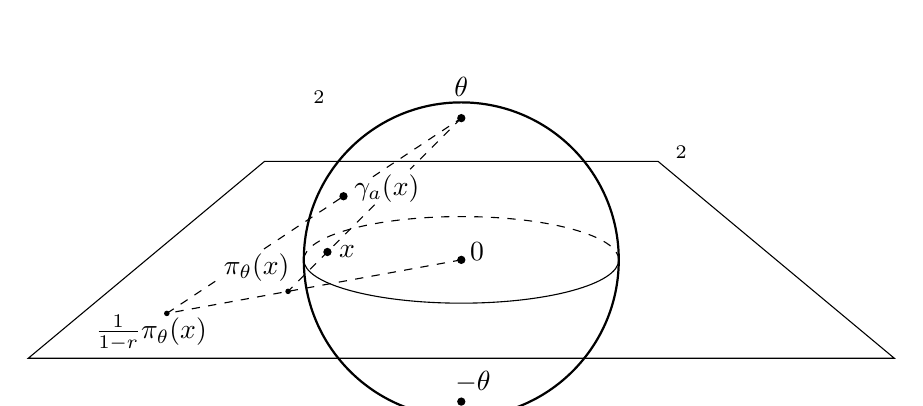
\begin{tikzpicture}
            %SFERA
            %linee
            \draw [thick] (0,0) circle (2);
            \draw (-2,0) arc (180:360: 2 and 0.55);
            \draw [dashed] (2,0) arc (0:180: 2 and 0.55);
            \fill (0,1.8) circle (1.5pt)
            (0,-1.8) circle (1.5pt)
            (-1.7,.1) circle (1.5pt)
            (0,0) circle (1.5pt)
            (-2.2,-.4) circle (1pt)
            (-2.2*1.7,-.4*1.7) circle (1pt)
            (-2.2*1.7*.4,-.4*1.7*.4-1.8*.4+1.8) circle (1.5pt);
            \draw[dashed] (0, 1.8) -- (-.65,1.15);
            \draw[dashed] (-1.1,.7)--(-2.2,-.4);
            \draw[dashed] (0,0) -- (-2.2*1.7,-.4*1.7);
            \draw[dashed] (-2.2*1.7,-.4*1.7)--(-2.2*1.7*.83,-.4*1.7*.83-1.8*.83+1.8);
            \draw[dashed] (-2.2*1.7*.67,-.4*1.7*.67-1.8*.67+1.8) -- (-2.2*1.7*.4,-.4*1.7*.4-1.8*.4+1.8);
            \draw[dashed] (-2.2*1.7*.3,-.4*1.7*.3-1.8*.3+1.8) -- (0, 1.8);

            %PIANO
            \draw (-5.5,-1.25) -- (5.5,-1.25) -- (2.5,1.25)--(-2.5,1.25)--cycle;
            
            %NOMI
            \node at (0,2.2){\(\theta\)};
            \node at (0.15,-1.55){\(-\theta\)};
            \node at (-2.6,-.1){\(\pi_{\theta}(x)\)};
            \node at (-2.2*1.7-.2,-.4*1.7-0.25) {\(\frac{1}{1-r}\pi_{\theta}(x)\)};
            \node at (-1.45,0.1){\(x\)};
            \node at (-2.2*1.7*.4+.55,-.4*1.7*.4-1.8*.4+1.8+.1){\(\gamma_a(x)\)};
            \node at (0.2,0.1){0};
            \node at (-1.8,2) {\(\Sp^2\)};
            \node at (2.8,1.3) {\(\R^2\)};
    \end{tikzpicture}
\caption{Construction of \(\gamma_a\).}
\end{figure}
    
Observe that for each \(\theta \in \Sp^2\)
\begin{equation}\label{eq: Hersch - key prop for extension to boundary}
	\lim_{a \to \theta}\gamma_a(x) = \theta \qquad \forall x \in \Sp^2\setminus\{-\theta\}.
\end{equation}
for each \(x \in \Sp^2\).
Now consider the map
\begin{equation*}
	\Psi \colon B^3 \to \R^3 
\end{equation*}
defined by 
\begin{equation*}
	\Psi(a) \coloneq \frac{1}{|\Sigma|}\int_\Sigma \gamma_a \circ \Phi \ \dif \sigma = \left( \frac{1}{|\Sigma|}\int_\Sigma x^i \circ \gamma_a \circ \Phi\ \dif \sigma \right)_{i=1,2,3} \qquad \forall a \in B^3
\end{equation*}
Clearly \(\Psi\) is a continuous function.

We need to show that there exists \(a_0 \in B^3\) such that \(\Psi(a_0)=0\), because then \(\gamma_{a_0}\) is the required conformal diffeomorphism. By triangular inequality, \(\Psi(B^3) \subset \overline{B^3}\): for any \(a \in B^3\)
\begin{equation*}
	\left| \frac{1}{|\Sigma|}\int_\Sigma \gamma_a \circ \Phi\ \dif \sigma \right| \le \frac{1}{|\Sigma|}\int_\Sigma |\gamma_a \circ \Phi| \dif \sigma  = 1.
\end{equation*}
By \eqref{eq: Hersch - key prop for extension to boundary}, for any \(\theta \in \Sp^2 = \de B^3\),
\[
	\lim_{a \to \theta} \frac{1}{|\Sigma|}\int_\Sigma \gamma_a \circ \Phi \ \dif \sigma =  \theta,
\]
so there exists a unique continuous extension \(\Psi \in C^0(\overline{B^3}, \overline{B^3})\) such that \(\Psi|_{\de B^3} = \Id_{B^3}\). 
To prove that \(0 \in \Psi(B^3)\), we can argue as in the classical proof of Brouwer fixed point theorem. We know that there is no retraction of \(\overline{B^3}\) on its boundary \(\de B^3\) (for example, because the homology group \(H_2(\de B^3) \cong \Z\) cannot be isomorphic to any subgroup of \(H_2(\overline{B^3})=0\)). Suppose by contradiction that \(0 \notin \Psi(\overline{B^3})\). Then we can define a retraction \(r \colon \overline{B^3} \to \de B^3 \) of \(\overline{B^3}\) on its boundary as:
	\[
		r(x) = \frac{\Psi(x)}{|\Psi(x)|},
	\]
a contradiction, so \(0 \in \Psi(\Sigma)\). This proves the lemma. \qedhere
\end{proof}

\appendix
\section{The Brill-Noether theorem}
A Riemann surface is a compact complex manifold of complex dimension 1, namely a complex curve. They correspond to all orientable closed surfaces: the sphere \(\Sp^2 = \C\Pbb^1\), the torus \(\T^2\) and the tori with multiple holes. The number of holes \(k\) is called \emph{genus}. 

Let \(\Sigma_1\) and \(\Sigma_2\) be two Riemann surfaces. A map \(\vp \colon \Sigma_1 \to \Sigma_2\) is holomorphic if on every complex atlas it's holomorphic. Fix two complex charts \((U, z)\) on \(\Sigma_1\) and \((V,w)\) on \(\Sigma_2\), and consider the local representation \(f=w \circ \vp \circ z^{-1} \colon \Omega \to \C\). Since \(f\) is holomorphic, its complex derivative \(f'\colon \Omega \to \C\) is still holomorphic, so it's either constantly 0 or it has a discrete set of zeroes. Moreover, by the Cauchy-Riemann equations, \(f \colon \Omega \to \R^2\) (as a real map) has only regular points and points where the differential vanishes. As a consequence, either \(\vp\) is constant, or it has a discrete set of critical points (and on those points, the differential \(\dif\vp\) vanishes), called \emph{branch points}. 

The complex structure implies strong geometric consequences. Indeed, it's not hard to prove the following.
\begin{prop}
    Let \((\Sigma_1,g_1)\) and \((\Sigma_2,g_2)\) be two Riemann surfaces (endowed with Riemannian metrics) and let \(\vp \colon \Sigma_1 \to \Sigma_2\) be a non constant holomorphic map. Then \(\vp \colon (\Sigma_1,g_1) \to (\Sigma_2,g_2)\) is almost-conformal, i.e. there exists a function \(\lambda \colon \Sigma_1 \setminus \Gamma \to \R\setminus\{0\}\) such that
    \[
        g_1 = \lambda^2 \vp^*g_2 \qquad \text{on }\Sigma_1\setminus \Gamma,
    \]
    where \(\Gamma\subset \Sigma_1\) is the set of branch points of \(\vp\). 
\end{prop}

It holds the following deep theorem (see \cite[Chapter XXI]{ACGH_GeometryAlgebraicCurves}).
\begin{thm}[Brill-Noether]\label{thm: Brill-Noether}
    Let \(\Sigma\) be a complex curve with genus \(k\). Then there exists a non degenerate\footnote{(A map \(\Phi \colon \Sigma \to \C\Pbb^r\) is \emph{degenerate} if the image is contained in some hyperplane \(\C\Pbb^{r-1}\subset \C\Pbb^r\).} map \(\Phi \colon \Sigma \to \C\Pbb^r\) of degree \(d\) if and only if
    \[
        \rho(d,r,k) = k-(r+1)(k-d+r) \ge 0.
    \]
\end{thm}

\begin{proof}[Proof of Theorem~\ref{thm: corollary of Brill-Noether}]
With the notation above, fix \(r=1\). Using the Brill-Noether Theorem, we can find the required map \(\Phi\) of degree \(d\) if and only if
\[
    0 \le \rho(d,1,k) = k-2(k-d+1) = 2d - (k+2),
\]
that is
\[
    d \ge 1 + \frac{k}{2}.
\]

Taking the \(d\) as the least possible value, we get
\[
d = \begin{cases}
    1 + k/2 &\text{if }k\text{ is even},\\
    3/2 + k/2 &\text{if }k\text{ is odd}.
\end{cases}
\]
Since \(\Phi \colon \Sigma \to \C\Pbb^1 = \Sp^2\) is non degenerate, it is not constant, so it has a discrete set of branch points \(\Gamma\). Since \(\Sigma\) is compact, \(\Gamma\) is finite. On \(\Sigma \setminus \Gamma\), \(\Phi\) is a local diffeomorphism, so \(\Phi \colon \Sigma \setminus \Gamma \to \Sp^2 \setminus \Phi(\Gamma)\) is a covering of degree equal to the degree of \(\Phi\) as a map. 

Finally, since \(\Phi\) is holomorphic, \(\Phi \colon (\Sigma, g) \to (\Sp^2,g_{\Sp^2})\) is almost-conformal, and more precisely it's conformal on \(\Sigma \setminus \Gamma\).
\end{proof}
\printbibliography
\end{document}
